%!TEX encoding = UTF-8 Unicode

\documentclass[landscape]{book}
\usepackage[a3paper]{geometry}

\usepackage{verbatim}

\usepackage{hyperref}

\usepackage{tikz}

\usetikzlibrary{
  arrows,
  shapes.misc,% wg. rounded rectangle
  shapes.arrows,%
  matrix,%
  scopes,%
  shadows%
}

\tikzset{
  nonterminal/.style={
    % The shape:
    rectangle,
    % The size:
    minimum size=6mm,
    % The border:
    very thick,
    draw=red!50!black!50,         % 50% red and 50% black,
                                  % and that mixed with 50% white
    % The filling:
    top color=white,              % a shading that is white at the top...
    bottom color=red!50!black!20, % and something else at the bottom
    % Font
    font=\itshape\small
  },
  terminal/.style={
    % The shape:
    rounded rectangle,
    minimum size=6mm,
    % The rest
    very thick,draw=black!50,
    top color=white,bottom color=black!20,
    font=\ttfamily\small
  },
  firstPoint/.style={circle,>=stealth',thick,draw=black!50},
  point/.style={coordinate,>=stealth',thick,draw=black!50},
  tip/.style={->,shorten >=0.007pt},
  lastPoint/.style={rectangle,>=stealth',thick,draw=black!50},
  every join/.style={rounded corners}
}

\newcommand\nonTerminalSection[2]{\section{Nonterminal \texttt{#1}}\label{nt:#2}}
\newcommand\ruleSubsection[3]{\subsection{Component \texttt{#1}, in file \texttt{#2}, line #3}}
\newcommand\ruleMatrixColumnSeparation{3mm}
\newcommand\ruleMatrixRowSeparation{3mm}
\newcommand\nonTerminalSymbol[2]{\hyperref[nt:#2]{#1}}
\newcommand\startSymbol[2]{The start symbol is \hyperref[nt:#2]{#1}.}

\newcommand\nonTerminalSummaryStart{This is the alphabetical list of non terminal : }
\newcommand\nonTerminalSummary[2]{\hyperref[nt:#2]{#1}}
\newcommand\nonTerminalSummarySeparator{, }
\newcommand\nonTerminalSummaryEnd{.\\}

\begin{document}

\title{\Huge{Grammar \texttt{galgas3ProjectGrammar}}}
\date \today 

\maketitle

\startSymbol{project\_component\_start\_symbol}{1}

\nonTerminalSummaryStart \nonTerminalSummary{project\_component\_start\_symbol}{1}\nonTerminalSummarySeparator \nonTerminalSummary{project\_header}{0}\nonTerminalSummaryEnd \nonTerminalSection{project\_component\_start\_symbol}{1}

\ruleSubsection{galgas3ProjectSyntax}{galgasProject}{64}

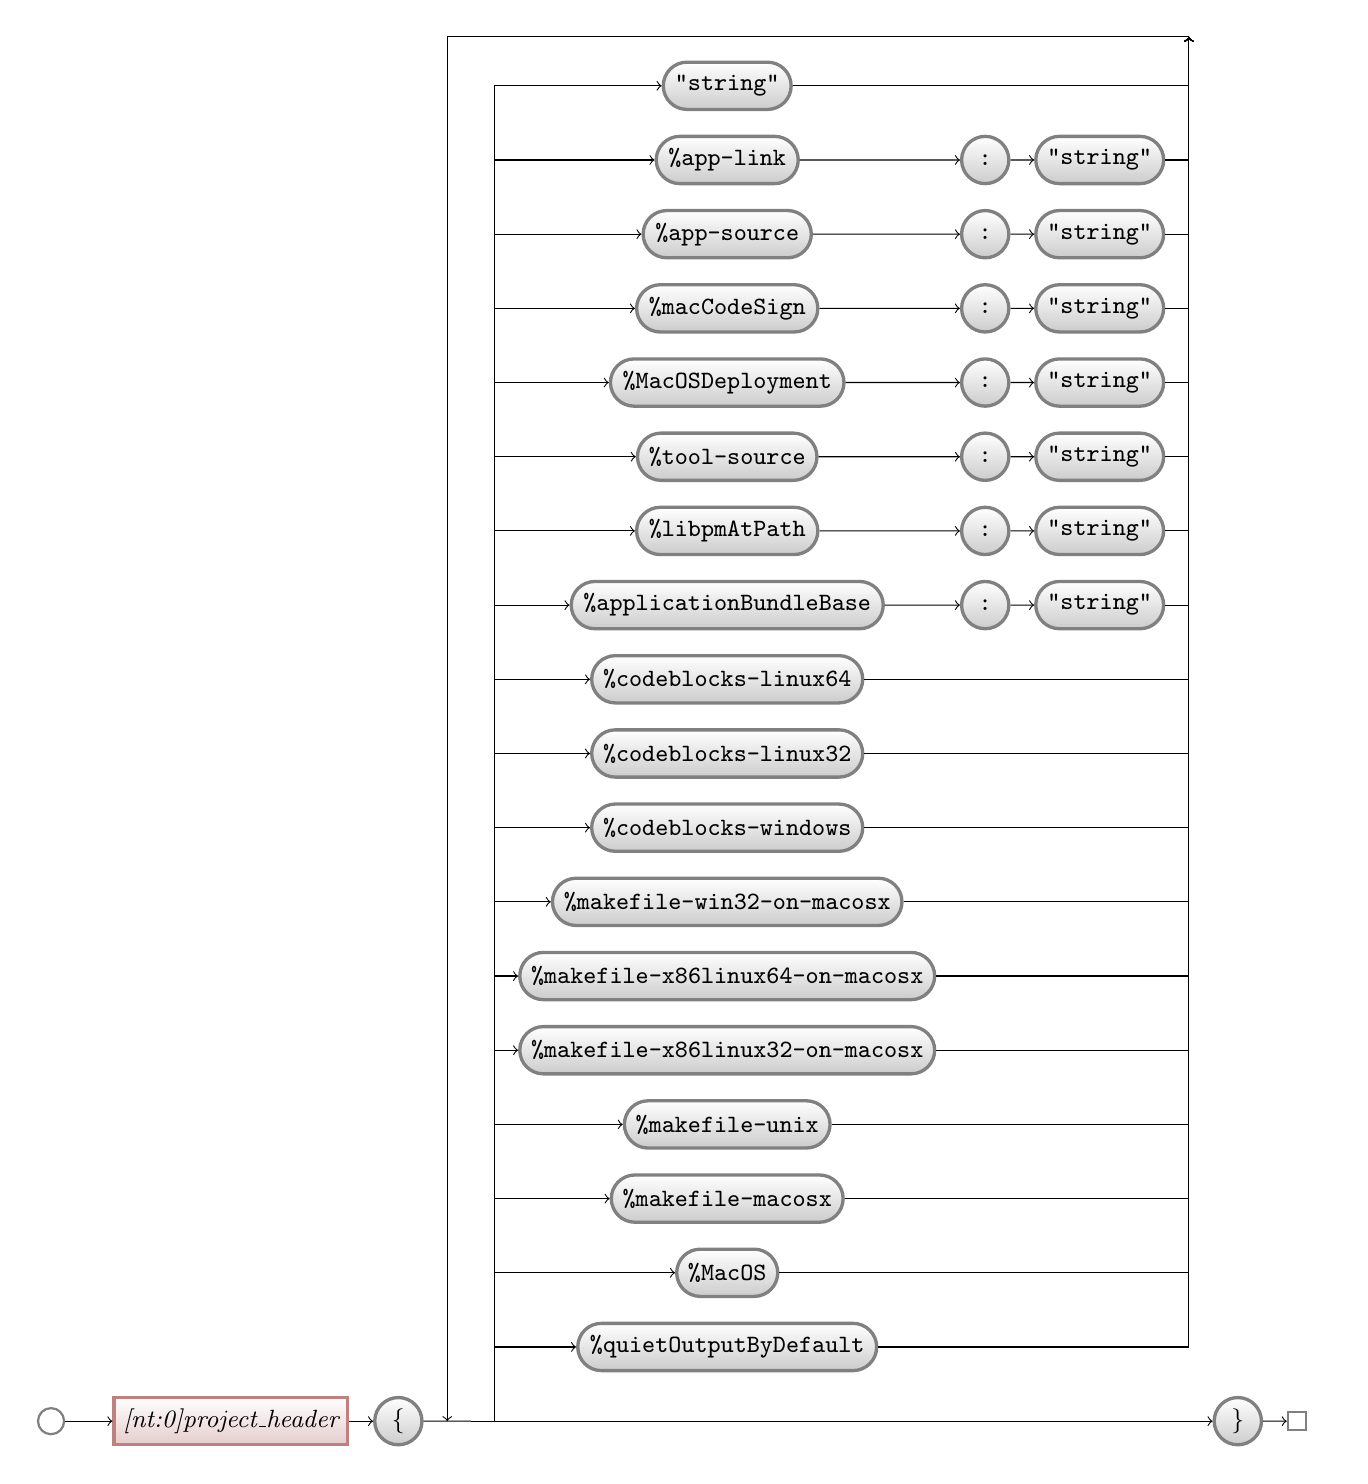
\begin{tikzpicture}
  \matrix[column sep=\ruleMatrixColumnSeparation, row sep=\ruleMatrixRowSeparation] {
    & & & & & & & & & & \node (p19-10) [point] {}; & \\
    & & & & & & & \node (p18-7) [terminal] {"string"}; & \\
    & & & & & & & \node (p17-7) [terminal] {\verb=%=app-link}; & \node (p17-8) [terminal] {:}; & \node (p17-9) [terminal] {"string"}; & \\
    & & & & & & & \node (p16-7) [terminal] {\verb=%=app-source}; & \node (p16-8) [terminal] {:}; & \node (p16-9) [terminal] {"string"}; & \\
    & & & & & & & \node (p15-7) [terminal] {\verb=%=macCodeSign}; & \node (p15-8) [terminal] {:}; & \node (p15-9) [terminal] {"string"}; & \\
    & & & & & & & \node (p14-7) [terminal] {\verb=%=MacOSDeployment}; & \node (p14-8) [terminal] {:}; & \node (p14-9) [terminal] {"string"}; & \\
    & & & & & & & \node (p13-7) [terminal] {\verb=%=tool-source}; & \node (p13-8) [terminal] {:}; & \node (p13-9) [terminal] {"string"}; & \\
    & & & & & & & \node (p12-7) [terminal] {\verb=%=libpmAtPath}; & \node (p12-8) [terminal] {:}; & \node (p12-9) [terminal] {"string"}; & \\
    & & & & & & & \node (p11-7) [terminal] {\verb=%=applicationBundleBase}; & \node (p11-8) [terminal] {:}; & \node (p11-9) [terminal] {"string"}; & \\
    & & & & & & & \node (p10-7) [terminal] {\verb=%=codeblocks-linux64}; & \\
    & & & & & & & \node (p9-7) [terminal] {\verb=%=codeblocks-linux32}; & \\
    & & & & & & & \node (p8-7) [terminal] {\verb=%=codeblocks-windows}; & \\
    & & & & & & & \node (p7-7) [terminal] {\verb=%=makefile-win32-on-macosx}; & \\
    & & & & & & & \node (p6-7) [terminal] {\verb=%=makefile-x86linux64-on-macosx}; & \\
    & & & & & & & \node (p5-7) [terminal] {\verb=%=makefile-x86linux32-on-macosx}; & \\
    & & & & & & & \node (p4-7) [terminal] {\verb=%=makefile-unix}; & \\
    & & & & & & & \node (p3-7) [terminal] {\verb=%=makefile-macosx}; & \\
    & & & & & & & \node (p2-7) [terminal] {\verb=%=MacOS}; & \\
    & & & & & & & \node (p1-7) [terminal] {\verb=%=quietOutputByDefault}; & \\
    \node (P0start) [firstPoint] {}; & & \node (p0-2) [nonterminal] {\nonTerminalSymbol{project\_header}{0}}; & \node (p0-3) [terminal] {\{}; & \node (p0-4) [point] {}; & \node (p0-5) [point] {}; & \node (p0-6) [point] {}; & & & & & \node (p0-11) [terminal] {\}}; & \node (p0-12) [lastPoint] {}; & \\
  };
  \draw[->] (P0start) -- (p0-2) ;
  \draw[->] (p0-2) -- (p0-3) ;
  \draw (p0-3) -- (p0-5) ;
  \draw[->] (p0-6) |- (p1-7) ;
  \draw[->] (p0-6) |- (p2-7) ;
  \draw[->] (p0-6) |- (p3-7) ;
  \draw[->] (p0-6) |- (p4-7) ;
  \draw[->] (p0-6) |- (p5-7) ;
  \draw[->] (p0-6) |- (p6-7) ;
  \draw[->] (p0-6) |- (p7-7) ;
  \draw[->] (p0-6) |- (p8-7) ;
  \draw[->] (p0-6) |- (p9-7) ;
  \draw[->] (p0-6) |- (p10-7) ;
  \draw[->] (p0-6) |- (p11-7) ;
  \draw[->] (p11-7) -- (p11-8) ;
  \draw[->] (p11-8) -- (p11-9) ;
  \draw[->] (p0-6) |- (p12-7) ;
  \draw[->] (p12-7) -- (p12-8) ;
  \draw[->] (p12-8) -- (p12-9) ;
  \draw[->] (p0-6) |- (p13-7) ;
  \draw[->] (p13-7) -- (p13-8) ;
  \draw[->] (p13-8) -- (p13-9) ;
  \draw[->] (p0-6) |- (p14-7) ;
  \draw[->] (p14-7) -- (p14-8) ;
  \draw[->] (p14-8) -- (p14-9) ;
  \draw[->] (p0-6) |- (p15-7) ;
  \draw[->] (p15-7) -- (p15-8) ;
  \draw[->] (p15-8) -- (p15-9) ;
  \draw[->] (p0-6) |- (p16-7) ;
  \draw[->] (p16-7) -- (p16-8) ;
  \draw[->] (p16-8) -- (p16-9) ;
  \draw[->] (p0-6) |- (p17-7) ;
  \draw[->] (p17-7) -- (p17-8) ;
  \draw[->] (p17-8) -- (p17-9) ;
  \draw[->] (p0-6) |- (p18-7) ;
  \draw[->] (p19-10) -| (p0-4) ;
  \draw[->] (p1-7) -| (p19-10) ;
  \draw[->] (p2-7) -| (p19-10) ;
  \draw[->] (p3-7) -| (p19-10) ;
  \draw[->] (p4-7) -| (p19-10) ;
  \draw[->] (p5-7) -| (p19-10) ;
  \draw[->] (p6-7) -| (p19-10) ;
  \draw[->] (p7-7) -| (p19-10) ;
  \draw[->] (p8-7) -| (p19-10) ;
  \draw[->] (p9-7) -| (p19-10) ;
  \draw[->] (p10-7) -| (p19-10) ;
  \draw[->] (p11-9) -| (p19-10) ;
  \draw[->] (p12-9) -| (p19-10) ;
  \draw[->] (p13-9) -| (p19-10) ;
  \draw[->] (p14-9) -| (p19-10) ;
  \draw[->] (p15-9) -| (p19-10) ;
  \draw[->] (p16-9) -| (p19-10) ;
  \draw[->] (p17-9) -| (p19-10) ;
  \draw[->] (p18-7) -| (p19-10) ;
  \draw[->] (p0-5) -- (p0-11) ;
  \draw[->] (p0-11) -- (p0-12) ;
\end{tikzpicture}

\nonTerminalSection{project\_header}{0}

\ruleSubsection{galgas3ProjectSyntax}{galgasProject}{49}

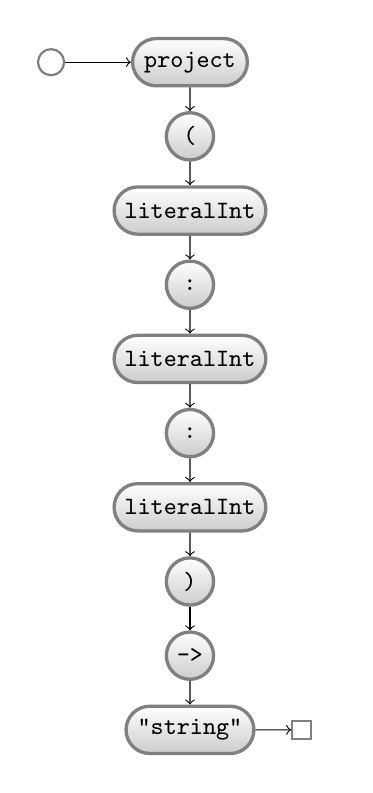
\begin{tikzpicture}
  \matrix[column sep=\ruleMatrixColumnSeparation, row sep=\ruleMatrixRowSeparation] {
    \node (P0start) [firstPoint] {}; & & \node (p9-2) [terminal] {project}; & \\
    & & \node (p8-2) [terminal] {(}; & \\
    & & \node (p7-2) [terminal] {literalInt}; & \\
    & & \node (p6-2) [terminal] {:}; & \\
    & & \node (p5-2) [terminal] {literalInt}; & \\
    & & \node (p4-2) [terminal] {:}; & \\
    & & \node (p3-2) [terminal] {literalInt}; & \\
    & & \node (p2-2) [terminal] {)}; & \\
    & & \node (p1-2) [terminal] {->}; & \\
    & & \node (p0-2) [terminal] {"string"}; & \node (p0-3) [lastPoint] {}; & \\
  };
  \draw[->] (P0start) -- (p9-2) ;
  \draw[->] (p9-2) -- (p8-2) ;
  \draw[->] (p8-2) -- (p7-2) ;
  \draw[->] (p7-2) -- (p6-2) ;
  \draw[->] (p6-2) -- (p5-2) ;
  \draw[->] (p5-2) -- (p4-2) ;
  \draw[->] (p4-2) -- (p3-2) ;
  \draw[->] (p3-2) -- (p2-2) ;
  \draw[->] (p2-2) -- (p1-2) ;
  \draw[->] (p1-2) -- (p0-2) ;
  \draw[->] (p0-2) -- (p0-3) ;
\end{tikzpicture}



\end{document}
